% This is samplepaper.tex, a sample chapter demonstrating the
% LLNCS macro package for Springer Computer Science proceedings;
% Version 2.20 of 2017/10/04
%
\documentclass[runningheads]{llncs}
%
\usepackage{graphicx}
\usepackage{hyperref}
\usepackage{amsthm}
% Used for displaying a sample figure. If possible, figure files should
% be included in EPS format.
%
% If you use the hyperref package, please uncomment the following line
% to display URLs in blue roman font according to Springer's eBook style:
% \renewcommand\UrlFont{\color{blue}\rmfamily}

\begin{document}
\newtheorem{defi}[theorem]{Definition}
\newtheorem*{prel}{Preliminaries}
%
\title{G2GML: Graph to Graph Mapping Language for Bridging RDF and Property Graphs}
%
\titlerunning{G2GML: Graph to Graph Mapping Lanugage}
%\titlerunning{Interoperable Use of RDF and Property Graph}
% If the paper title is too long for the running head, you can set
% an abbreviated paper title here
%
\author{Hirokazu Chiba\inst{1} \and Ryota Yamanaka\inst{2} \and Shota Matsumoto\inst{3}}
%
\authorrunning{H. Chiba {\itshape et al.}}
% First names are abbreviated in the running head.
% If there are more than two authors, 'et al.' is used.
%
\institute{
Database Center for Life Science, Chiba 277-0871, Japan\\
\email{chiba@dbcls.rois.ac.jp}
\and
Oracle Corporation, Bangkok 10500, Thailand\\
\email{ryota.yamanaka@oracle.com}
\and
Lifematics Inc., Tokyo 101-0041, Japan\\
\email{shota.matsumoto@lifematics.co.jp}
}
%
\maketitle              % typeset the header of the contribution
%
\begin{abstract}
% The abstract should briefly summarize the contents of the paper in 15--250 words.
How can we maximize the value of accumulated RDF data? Although increasing amounts of scientific and social data are described as RDF, their use cases are still limited. Allowing access to the RDF datasets through various interface beyond the SPARQL interface will be expected. Importing the RDF datasets into various graph analysis engines will increase the values of the datasets.  
However, interoperable management of such graph data is challenging due to the differences in existing models and formats depending on various implementations. Here, we redefine the property graph model incorporating the differences in existing models and propose exchangeable serialization formats for property graphs, which can be converted into specific formats for each of the databases. 
The serialization formats independent of certain database implementations will increase the interoperability of graph databases and will make it easier for users to import accumulated graph data.
We further propose a framework for mapping RDF graphs to property graphs on the basis of the Graph to Graph Mapping Language (G2GML). Using this framework, accumulated graph data described in RDF can be converted to property graphs, which can then be loaded into several graph database engines for further analysis. 
%This work provides interoperability not only between property graph formats but also between RDF and proper graphs.
%Future works include implementing and utilizing graph algorithms to make the most of the accumulated data in various analytical engines.

\keywords{RDF \and Property Graph \and Graph Database}
\end{abstract}

\section{Introduction}
% Please note that the first paragraph of a section or subsection is not indented. The first paragraph that follows a table, figure, equation etc. does not need an indent, either.

Increasing amounts of scientific and social data are published in the form of Resource Description Framework (RDF)~\cite{rdf}. It now constitutes a large open data cloud. DBpedia~\cite{dbpedia} and Wikidata~\cite{wikidata} are good example. SPARQL~\cite{sparql} is a standardized interface for RDF. However, the usecases through thouse interface are still limited. Although the standardized format and interface contributed the integrated large data could, further interface is expected to maximize the value of RDF datasets. 
% Although RDF data can be queried using the SPARQL language~\cite{sparql} in a flexible way, SPARQL is not dedicated to traversal of graphs and has a limitation in implementing graph analysis algorithms.
Recently, the property graph model~\cite{angles1,angles2} have been attracting increasing attention in the context of graph analysis; various graph database engines, including Neo4j~\cite{neo4j}, Oracle Labs PGX~\cite{pgx}, and Amazon Neptune~\cite{neptune}, adopt this model. These graph database engines support algorithms for traversing or analyzing graphs. However, currently not many datasets are consistently described in the property graph model, so the application of these powerful engines are limited.

Considering this situation, it is valuable to develop a method to transform RDF into property graphs. One of the practical issues is the lack of a standardized model for property graphs. 
Another issue is that transformation between them is not straightforward due to the differences between RDF and property graph models. 
In RDF graphs, all information is expressed as the triple (node-edge-node), whereas in property graphs, arbitrary information can be contained in each of the nodes and edges as the key-value form. 
Although this issue has been previously addressed on the basis of predefined transformations~\cite{hartig},
users still cannot control the mapping for their specific use cases.

Here, we redefine the property graph model incorporating the differences in existing models and also propose serialization formats based on the data model. We further propose a graph to graph mapping framework on the basis of the Graph to Graph Mapping Language (G2GML). Using this mapping framework, accumulated graph data described in RDF can be converted into property graphs, which can then be loaded into several graph database engines for further analysis. We will show several use cases where publicly available RDF data is extracted and convert to property graphs and also evaluate the performance. This work provides the foundation of interoperability of knowledge graphs.

The contributions of this papers are 1) development of Graph to Graph Mapping Language 2) proposal of common property graph model and serialization 3) development of G2G mapper 4) construction of knowledge graph resources in a common format as Graph Archive.


%%%%%%%%%%%%%%%%%%%%%%%
\section{G2G: Graph to Graph Mapping Framework}

\subsection{Overview}

Here we illustrate the overview of the framework.
G2G is a framework to describe mapping between RDF and property graphs for interoperable use of them. In this framework, users can specify mappings from RDF to property graphs in G2GML.
This mapping is processed by a tool called G2G Mapper, which was implemented by authors (available on \url{https://github.com/g2glab/g2g}). This tool can convert RDF data retrieved from SPARQL endpoints or from local files into PG format and then into specific formats for each of the database implementations.

The G2GML is a declarative language which consists of pairs of RDF graph patterns and property graph patterns. 
An intuitive meaning of a G2GML description is a map from  RDF subgraphs that matches the specified patterns to specified components of property graphs.

As an entry point to property graph, we define the Property Graph format, which is based on the Property Graph model.



%%%%%%%%%%%%%%%%%%
\subsection{G2GML}

G2GML is a language to describes maps from RDF graphs to Property graphs (PG). G2GML is a domain specific declarative language where programmers only have to describe target patterns of RDF and PG. RDF pattern is described using SPARQL pattern, and PG pattern is described using Cypher pattern.

\begin{prel}
An RDF triple $(s, p, o)$ is an element of $(I \cup B) \times I \times (I \cup B \cup L)$ where $I$, $L$ and $B$ are a set of IRIs, a set of literals and a set of blank nodes, which are considered pairwise disjoint. In this paper, an RDF triple is simply called a triple. For a triple $(s, p, o)$, $s$ is called the subject, $p$ the predicate and $o$ the object. An RDF graph is defined as a finite set of triples.
\end{prel}

\par
In this paper, we call maps written in G2GML as \textit{G2G maps}.
A \textit{G2G map} consists of one or more \textit{node maps} and \textit{edge maps}.
A \textit{node map} is a function that maps from an RDF graph to a set of \textit{PG nodes}. 
Similarly, an \textit{edge map} is a function that maps from an RDF graph to a set of \textit{PG edges}.
The meaning of a G2G map is a function that maps from an RDF graph to a set of PG nodes and edges that is mapped by  all its node and edge maps. We show a complete example of G2GML in Figure \ref{fig:example-g2g}.
%TODO: consider the position of the example
A node map is described as a pair of a PG node pattern  and an RDF graph pattern. Here we define the syntax of PG node pattern as follows. Note that symbols in uppercase are implicitly identifiers.
\begin{defi}[EBNF notation of PG node pattern]
\leavevmode
\begin{verbatim}
 node_pat  ::= "(" NODE  ":" LABEL  ("{" prop_list "}")? ")"
 prop_list ::= property "," prop_list | property
 property  ::= PROP_NAME ":" PROP_VAL
\end{verbatim}
\end{defi}

A PG node pattern specifies a node, a label and properties to be generated by the map. The \texttt{NODE} symbol specifies ID of the generated node, which is replaced by the resource retrieved by RDF graph. The \texttt{LABEL} symbol specifies the label of the resultant node. A label also works as the name of the node map which is referred from edge maps.
Therefore an identifier of a label must be unique in a  G2GML map.
Each node pattern contains zero or more properties as \texttt{prop\_list}.
A \texttt{property} is a pair of \texttt{PROP\_NAME} and \texttt{PROP\_VAL} that describes properties of nodes.
Identifiers \texttt{NODE} and \texttt{PROP\_VAL} must be names of variables in the succeeding RDF graph pattern, while \texttt{LABEL} and \texttt{PROP\_NAME} are regarded as text literals.

An RDF graph pattern in G2GML can be written in \textit{GroupGraphPattern} in SPARQL syntax (see EBNF notation of SPARQL grammer~\cite{sparql}).
An RDF graph pattern specifies which resources should be mapped to PG nodes. Resources matching with these pattern yield solution sets of SELECT query in SPARQL, which 
 are mapped to PG nodes by embedding variable bindings to corresponding location according to the preceding PG node pattern.
Here, a variable bound to \texttt{PROP\_VAL} may have multiple candidates for single node. If such multiple candidate exists, they are concatenated into an array in the manner of \texttt{GROUP\_CONCAT} in SPARQL if multiple resources are bound to single \texttt{PROP\_NAME}.

A PG edge pattern specifies a pattern of edge, the label, the properties and the source node and the destination node.
Here we define the syntax of PG edge pattern as follows.
\begin{defi}[EBNF notation of PG edge pattern]
\leavevmode
\begin{verbatim}
edge_pat ::= "(" SRC  ":" SRC_LAB ") -" 
                "[" EDGE?  ":" EDGE_LAB  ("{" prop_list "}")? ")" 
                ("->" | "-") "(" DST ":" DST_LAB ")"
\end{verbatim}
\end{defi}

 Identifiers of \texttt{SRC} and \texttt{DST} specify which variables in the succeeding RDF graph pattern should be mapped to endpoint nodes of resultant edges.
A \texttt{SRC\_LAB} and a \texttt{DST\_LAB} work not only as labels of resultant nodes but also work as implicit constraints of the edge map.
%TODO add ref
The resultant source nodes and destination nodes must match patterns in corresponding node maps.
For this reason, \texttt{SRC\_LAB} and \texttt{DST\_LAB} must be defined in other node maps.
\texttt{EDGE}, \texttt{EDGE\_LAB} and \texttt{prop\_list} can be described in the same manner as those counterparts in node maps.

The primary key of an edge map is the tuple of the resources bound to \texttt{SRC}, \texttt{EDGE} and \texttt{DST}. As well as node maps, other values of properties bound in \texttt{prop\_list} are concatenated into an array. 

The resultant edges can be either directed or undirected. If we use '\texttt{->}' as delimiter between an edge part and a destination part, the edge will be a directed edge.
 %TODO: add whole syntax of G2G using PG node pattern and edge pattern and SPARQL

%%%%%%%%%%%
\subsection{The Property Graph Model}
Here we define the property graph model independent of specific graph database implementations. For the purpose of interoperability, we incorporate differences in property graph models, taking into consideration multiple labels or property values for nodes and edges, as well as mixed graphs with both of directed and undirected edges. The property graph model we redefine here requires the following characteristics:

\begin{itemize}
    \item A property graph contains nodes and edges.
    \item Each of the nodes and edges can have zero or more labels.
    \item Each of the nodes and edges can have properties (key-value pairs).
    \item Each property can have multiple values.
    \item Each edge can be directed or undirected.
\end{itemize}
More formally, we define the property graph model as follows.

\begin{defi}[Property Graph Model]
\leavevmode \vspace{1mm} \\
A \emph{Property Graph} is a tuple
$PG = \langle N, E_d, E_u, S, V, P, e, l_n, l_e, p_n, p_e\rangle$, where:
\begin{enumerate}
    \item $N$ is a set of nodes.
    \item $E_d$ is a set of directed edges.
    \item $E_u$ is a set of undirected edges.
    \item $E$ is a set of edges where $E = E_d \cup E_u$.
    \item $S$ is a set of strings.
    \item $V$ is a set of values of arbitrary data types.
    \item $P$ is a set of properties. Each property has the form $p = \langle k,v \rangle$, where $k \in S$ and $v \in 2^V$.
    \item $e: E \to \langle N \times N \rangle$ is a function which yields the endpoints of each directed or undirected edge (if the edge is directed, the first node is the source and the second node is the destination).
    \item $l_n : N \to 2^S$ is a function mapping each node to its multiple labels.
    \item $l_e : E \to 2^S$ is a function mapping each edge to its multiple labels.
    \item $p_n : N \to 2^P$ is a function used to assign nodes to their multiple properties.
    \item $p_e : E \to 2^P$ is a function used to assign edges to their multiple properties.
\end{enumerate}
\end{defi}


\subsection{Serialization of Property Graphs}
According to our definition of the property graph model, we propose serialization in flat text and JSON. The flat text format (PG) is better for human readability and line-oriented processing, while the JSON format (JSON-PG) is best used for server-client communication.

The flat text PG format has the following characteristics, and an example is given in Figure~\ref{fig:example-pg}.

\begin{itemize}
    \item Each line describes a node or an edge.
    \item All elements in each line are separated by space or tab.
    \item In each of the node lines, the first column contains the node ID.
    \item In each of the edge lines, the first three columns contain the source node ID, the direction, and the destination node ID.
    \item Each line can contain an arbitrary number of labels.
    \item Each line can contain an arbitrary number of properties (key-value pairs).
\end{itemize}

More formally, we describe the PG format in the EBNF notation as follows.

\begin{defi}[EBNF notation of the PG format]
\leavevmode
\begin{verbatim}
 pg         ::= (node | edge)+
 node       ::= NODE_ID labels properties NEWLINE
 edge       ::= NODE_ID direction NODE_ID labels properties NEWLINE
 labels     ::= label*
 properties ::= property*
 label      ::= ":" STRING
 property   ::= STRING ":" value
 value      ::= STRING | NUMBER
 direction  ::= "--" | "->"
\end{verbatim}
\end{defi}

Next, we describe the JSON-PG format which follows the JSON syntax in addition to the above definition of the property graph model. The JSON-PG format has the following characteristics, and an example of the format is shown in Figure~\ref{fig:example-json}. It is to be noted that, whereas the set of labels or property values are represented as arrays in JSON, those elements are supposed to have no specific order according to the property graph model.

\begin{itemize}
    \item Nodes and edges are listed under \texttt{nodes} and \texttt{edges} elements, respectively.
    \item Edge direction is defined with the boolean element \texttt{undirected}. By default it is false (directed).
    \item Labels are listed under the \texttt{labels} element.
    \item Properties (key-value pairs) are listed under the \texttt{properties} element.
\end{itemize}

Furthermore, we have implemented command-line tools to convert between PG and JSON-PG, as well as to transform them into formats for well-known graph databases such as Neo4j, Oracle Labs PGX, and Amazon Neptune. The practical use cases of our tools demonstrate that the proposed data model and formats have the capability to describe property graph data begin used in existing graph databases (see \url{https://github.com/g2glab/pg}).

\begin{figure}[!t]
\begin{scriptsize}
\begin{verbatim}
# NODES
101  :Person  name:Alice  age:15  country:"United States"
102  :Person  :Student  name:Bob  country:Japan  country:Germany

# EDGES
101 -- 102  :sameSchool  :sameClass  since:2012
102 -> 101  :likes  since:2015
\end{verbatim}
\end{scriptsize}
\caption{Example of PG}
\label{fig:example-pg}
\end{figure}

\begin{figure}[!t]
\begin{scriptsize}
\begin{verbatim}
{
  "nodes":[
    {
     "id":101,
     "labels":["Person"],
     "properties":{"name":["Alice"], "age":[15], "country":["United States"]}
    },
    {
     "id":102,
     "labels":["Person", "Student"],
     "properties":{"name":["Bob"], "country":["Japan", "Germany"]}
    }
  ],https://ja.overleaf.com/project/5d6e87b11a254100014e487d
  "edges":[
    {
     "from":101,
     "to":102,
     "undirected":true,
     "labels":["sameSchool", "sameClass"],
     "properties":{"since":[2012]}
    },
    {
     "from":102,
     "to":101,
     "labels":["likes"],
     "properties":{"since":[2015]}
    }
  ]
}
\end{verbatim}
\end{scriptsize}
\caption{Example of JSON-PG}
\label{fig:example-json}
\end{figure}

%%%%%%%%%%%%
\subsection{Minimal Exmples}
Figure~\ref{fig:example-g2g} shows the small example of G2G mapping from RDF data to PG data. This example shows the following five types of the typical mapping.

\begin{itemize}
    \item Resource to node: In the line 2-4, the RDF resources with type \texttt{:Person} are mapped into PG nodes using their URIs as node IDs.
    \item Datatype property to node property: In the line 2-4, the RDF datatype property \texttt{:name} is mapped into PG node property key \texttt{name}. The literal objects 'Alice' and 'Bob' are mapped into the node property values.
    \item Object property to edge: In the line 5-6, the RDF object property \texttt{:likes} is mapped into PG edge \texttt{follows}. 
    \item Resource to edge: In the line 7-10, the RDF resource with type \texttt{:Follow} is mapped into PG edge \texttt{follows}. 
    \item Datatype property to edge property: In the line 7-10, the RDF datatype property \texttt{:since} is mapped into PG edge property \texttt{since}. The literal objects \texttt{2017} is mapped into the edge property value.
\end{itemize}


\begin{figure}[!t]
\begin{scriptsize}
\begin{verbatim}
@prefix : <http://example.org/> .
:person1 a :Person ;
         :name 'Alice' .
:person2 a :Person ;
         :name 'Bob' .
:person1 :supervised_by :person2 .
[] a :Email ;
   :sender     :person1 ;
   :receiver   :person2 ;
   :year       2017 .
   :attachment '01.pdf'
\end{verbatim}
\end{scriptsize}
\caption{Example of input RDF data}
\label{fig:example-rdf}
\end{figure}


\begin{figure}[!t]
\begin{scriptsize}
\begin{verbatim}
PREFIX : <http://example.org/>
(p:Person {name:n})
    ?p a :Person .
    ?p :name ?n .
(p1:Person)-[:supervised_by]->(p2:Person)
    ?p1 :supervised_by ?p2 .
(p1:person)-[:emailed {year:y, attachment:a}]->(p2:person)
    ?f :sender   ?p1 ;
       :receiver ?p2 ;
       :year     ?y .
    OPTIONAL { ?f :attachment ?a }
\end{verbatim}
\end{scriptsize}
\caption{Example of G2G mapping definition}
\label{fig:example-g2g}
\end{figure}


\begin{figure}[!t]
\begin{scriptsize}
\begin{verbatim}
"http://example.org/person1" :person name:Alice
"http://example.org/person2" :person name:Bob
"http://example.org/person1" -> "http://example.org/person2" :supervised_by
"http://example.org/person1" -> "http://example.org/person2" :emailed year:2017 attachment:"01.pdf"
\end{verbatim}
\end{scriptsize}
\caption{Example of output PG data}
\label{fig:example-pg}
\end{figure}


\begin{figure}
\center
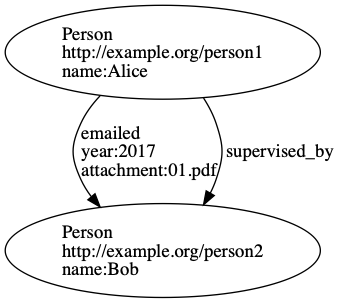
\includegraphics[width=0.5\textwidth]{pg_example5.png}
\caption{Example of created PG}
\label{fig:pg_example5}
\end{figure}


%%%%%%%%%%%
\subsection{Mapping Details}
The G2G mapping based on G2GML is generally intuitive as it is shown above, however, there are several discussions about the details of mapping.


\subsubsection{Multi Edges}
When a pair of RDF resources has multiple relationships, those will be converted not to a single PG edge with multiple properties but to multiple PG edges. The G2GML in Figure~\ref{fig:example-g2g} generates two PG edges for the RDF data in Figure~\ref{fig:example-rdf2} for keeping the information that Alice emailed Bob twice.


\begin{figure}[!t]
\begin{scriptsize}
\begin{verbatim}
@prefix : <http://example.org/> .
:person1 a :Person ;
         :name 'Alice' .
:person2 a :Person ;
         :name 'Bob' .
[] a :Email ;
   :sender   :person1 ;
   :receiver :person2 ;
   :year     2017 .
[] a :Email ;
   :sender   :person1 ;
   :receiver :person2 ;
   :year     2018 .
\end{verbatim}
\end{scriptsize}
\caption{Example of input RDF data (multi edges)}
\label{fig:example-rdf2}
\end{figure}


\begin{figure}[!t]
\begin{scriptsize}
\begin{verbatim}
"http://example.org/person1" :Person name:Alice
"http://example.org/person2" :Person name:Bob
"http://example.org/person1" -> "http://example.org/person2" :emailed year:2017
"http://example.org/person1" -> "http://example.org/person2" :emailed year:2018
\end{verbatim}
\end{scriptsize}
\caption{Example of output PG data (multi edges)}
\label{fig:example-pg2}
\end{figure}

\subsubsection{List of Property Values}
Each PG property can have multiple values. When a RDF resource has the same data property multiple times, the values are assumed to be the members of a list. The G2GML in Figure~\ref{fig:example-g2g} generates one PG edge with two properties for the RDF data in Figure~\ref{fig:example-rdf3} keeping the information that Alice emailed Bob once and it had two attachments.


\begin{figure}[!t]
\begin{scriptsize}
\begin{verbatim}

@prefix : <http://example.org/> .
:person1 a :Person ;
         :name 'Alice' .
:person2 a :Person ;
         :name 'Bob' .
[] a :Email ;
   :sender     :person1 ;
   :receiver   :person2 ;
   :year       2017 ;
   :attachment '01.pdf' ;
   :attachment '02.pdf' .

\end{verbatim}
\end{scriptsize}
\caption{Example of input RDF data (list of property values)}
\label{fig:example-rdf3}
\end{figure}


\begin{figure}[!t]
\begin{scriptsize}
\begin{verbatim}

"http://example.org/person1" :Person name:Alice
"http://example.org/person2" :Person name:Bob
"http://example.org/person1" -> "http://example.org/person2" :emailed year:2017 attachment:"01.pdf" attachment:"02.pdf"

\end{verbatim}
\end{scriptsize}
\caption{Example of output PG data (list of property values)}
\label{fig:example-pg3}
\end{figure}


%%%%%%%%%%%%%%%%%%%%%%%%%%%%%%%%%%%%%%%%%%%%%%%%%%%%%%%%%%%%%%%%%%%%%%%%%%%%%%%%%%%%%%%%%%%%%

\section{Use Cases}
 
We present several use cases to show how to applythe usefulness of G2G mapping framework, where we utilizeuse publicly available open data available in RDF datasets through SPARQL endpoints.
 
Figure~\ref{fig:dataflow} shows the overview of the mapping.
In this framework, users can specify mappings from RDF to property graphs in G2GML.
This mapping is processed by a tool called G2G Mapper, which was implemented by authors (available on \url{https://github.com/g2glab/g2g}). This tool can convert RDF data retrieved from SPARQL endpoints or from local files into PG format and then into specific formats for each of the database implementations.
 
The G2GML is a declarative language which consists of pairs of RDF graph patterns and property graph patterns. 
An intuitive meaning of a G2GML description is mapping RDF subgraphs that matches the specified patterns to specified components of property graphs.
 
 
\begin{figure}
\center
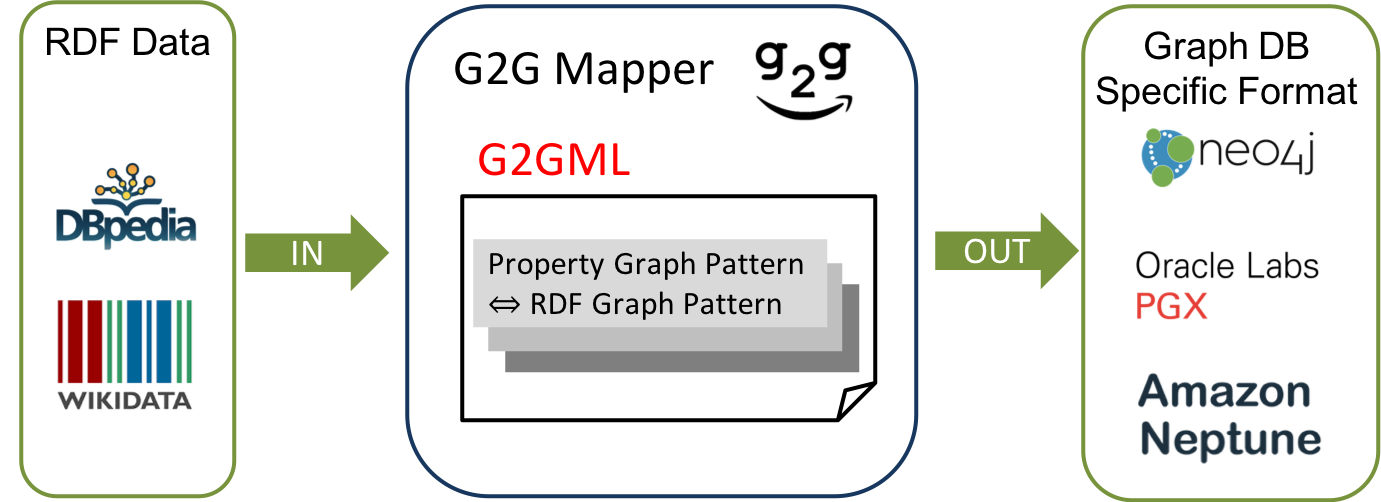
\includegraphics[width=1.0\textwidth]{dataflow.png}
\caption{Overview of the mapping from RDF to property graph}
\label{fig:dataflow}
\end{figure}
 
\subsection{Using Wikidata}
 
Here we present use case of for Wikidata. Wikidata is a useful source of biological open data, and it is available in the form of RDF through the SPARQL interface.
 
In Wikidata, each disease is associated with zero or more genes and drugs.
The subset of Wikidata can be extracted using G2G framework by writing a mapping file in G2GML (see the following list).
Here, we focus on human genes. So we specified the necessary conditions in G2GML.
Each entity of ‘Q12136: disease’ can have property ‘P2176: drug used for treatment’, thereby linked to items of ‘Q12140: medication’. Also, each disease can have property ‘P2293: genetic association’, thereby linked to items of ‘Q7186: gene’.
 
The numbers of obtained entities are as follows.
 
4689 diseases
4495 human genes
1285 drugs
 
The following figure shows the schematic relationships between those entities.
 
\begin{figure}
\center
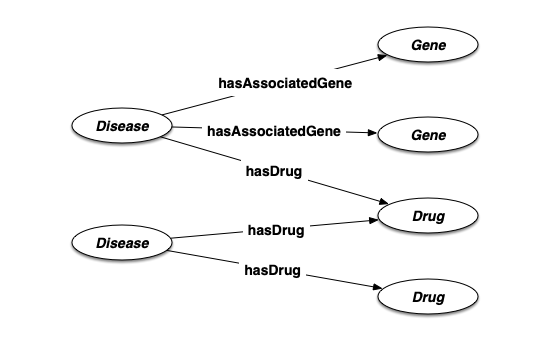
\includegraphics[width=0.7\textwidth]{wikidata_schema.png}
\caption{Schematic relation of Wikidata entities}
\label{fig:wikidata_schema.png}
\end{figure}
 
%--code--code--code--code--code--
\begin{figure}[!t]
\vspace{2mm}
\begin{scriptsize}
\begin{verbatim}
 
PREFIX wd: <http://www.wikidata.org/entity/>
PREFIX wdt: <http://www.wikidata.org/prop/direct/>
 
(g:HumanGene {symbol: s})
    ?g wdt:P31 wd:Q7187 ;      # instance of gene
       wdt:P703 wd:Q15978631 ; # found in taxon Homo sapiens
       wdt:P353 ?s .           # HGNC gene symbol
 
(d:Disease {name: n})
    ?d wdt:P31 wd:Q12136 ;     # instance of disease
       rdfs:label ?l .
    FILTER(lang(?l) = "en")
    BIND(str(?l) AS ?n)
 
(m:Drug {name: n})
    ?m wdt:P31 wd:Q12140 ;     # instance of medication
       rdfs:label ?l .
    FILTER(lang(?l) = "en")
    BIND(str(?l) AS ?n)
 
(d:Disease)-[:hasAssociatedGene]->(g:HumanGene)
    ?d wdt:P2293 ?g .          # genetic association
 
(d:Disease)-[:hasDrug]->(m:Drug)
    ?d wdt:P2176 ?m .          # drug used for treatment
 
\end{verbatim}
\end{scriptsize}
\caption{G2GML for Wikidata extraction}
\label{fig:g2gml_wikidata}
\end{figure}
%--code--code--code--code--code--
 
\begin{figure}
\center
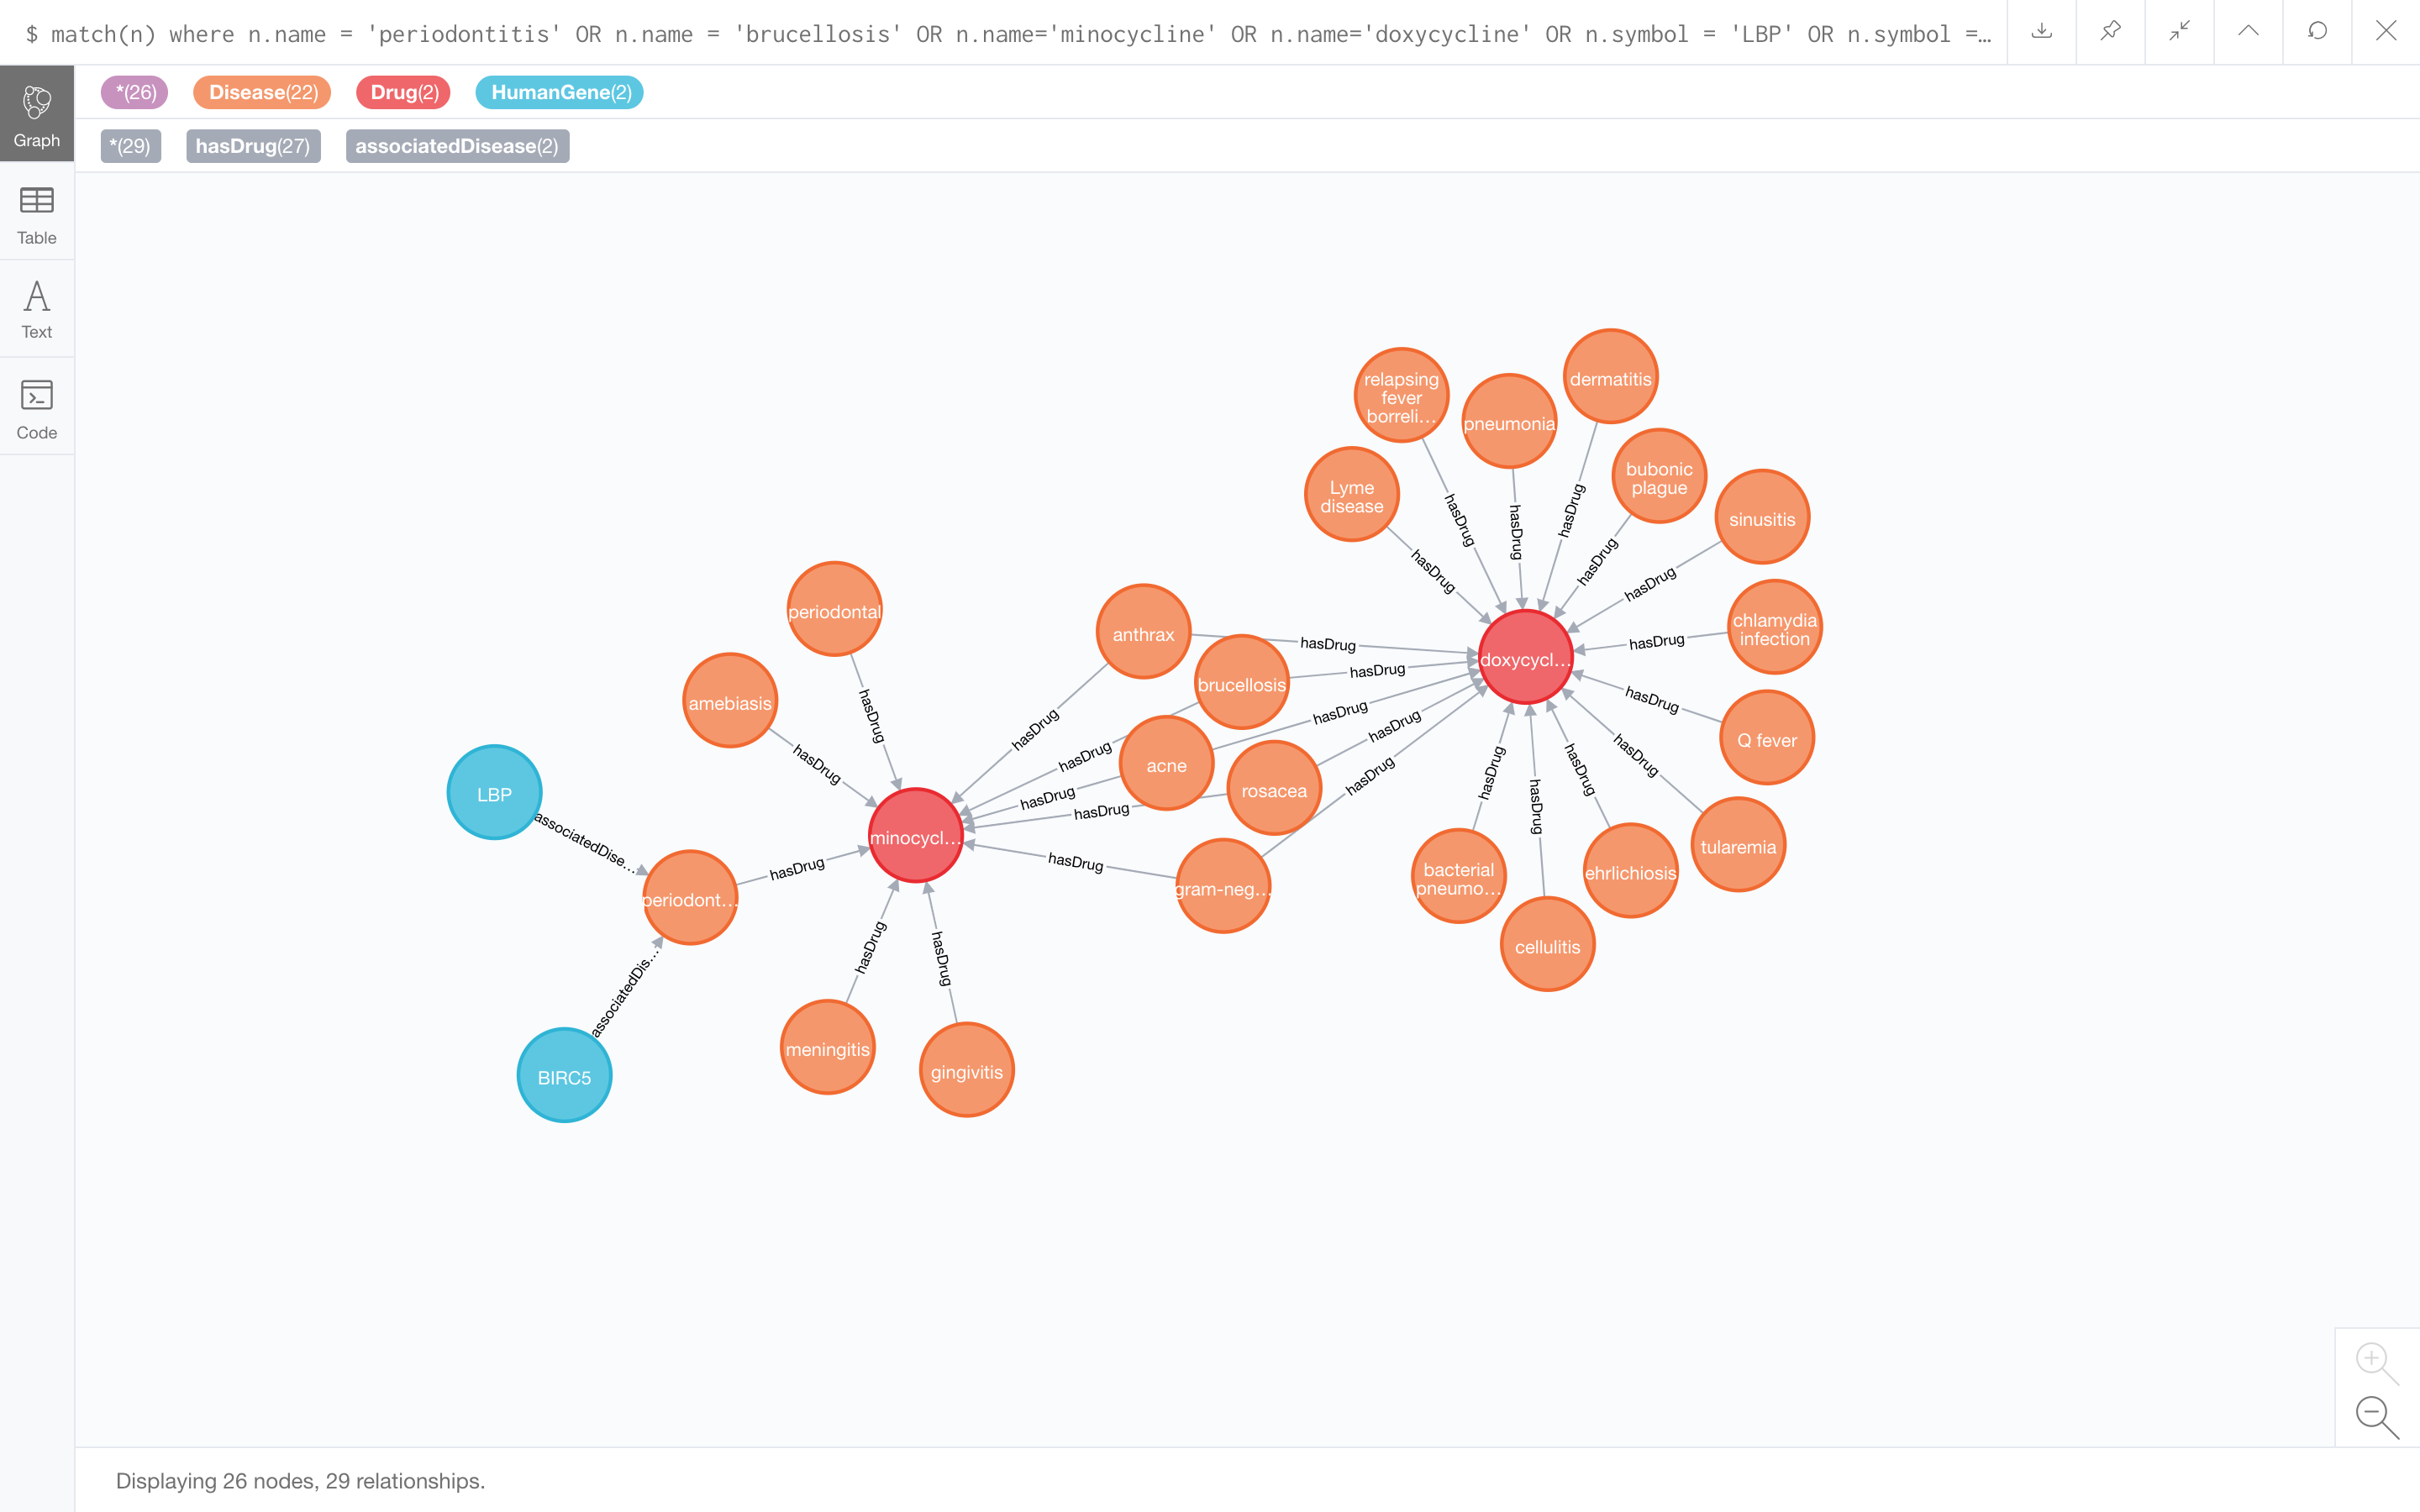
\includegraphics[width=1.0\textwidth]{neo4jexample2.png}
\caption{Visualization on Neo4j}
\label{fig:neo4jexample2.png}
\end{figure}
 
\subsection{Using DBpedia}
 
Here we describe a framework for mapping RDF graphs to property graphs.
Figure~\ref{fig:dataflow} shows the overview of the framework.
In this framework, users can specify mappings from RDF to property graphs in G2GML.
This mapping is processed by a tool called G2G Mapper, which was implemented by authors (available on \url{https://github.com/g2glab/g2g}). This tool can convert RDF data retrieved from SPARQL endpoints or from local files into PG format and then into specific formats for each of the database implementations.
 
The G2GML is a declarative language which consists of pairs of RDF graph patterns and property graph patterns. 
An intuitive meaning of a G2GML description is mapping RDF subgraphs that matches the specified patterns to specified components of property graphs. 
 
Figure~\ref{fig:conversion} schematically shows an example of the G2G mapping to convert RDF data retrieved from DBpedia into property graph data. 
When we focus on a relationships where two musicians (\texttt{?m1} and \texttt{?m2}) belong to the same group, such information can be represented in the property graph shown in the right side of the figure.
 
\begin{figure}
\center
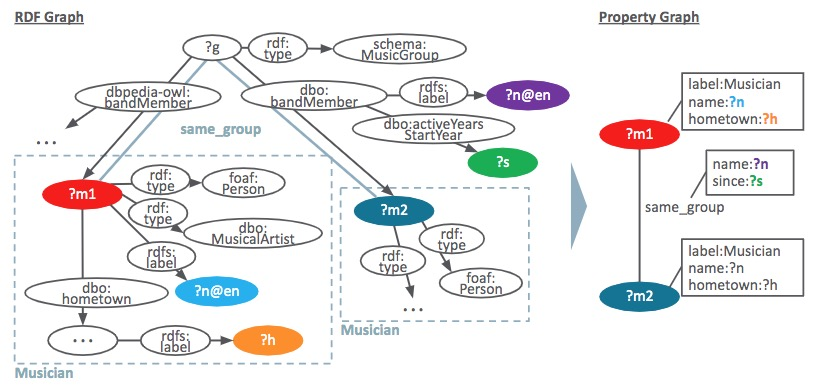
\includegraphics[width=1.0\textwidth]{example.jpg}
\caption{Schematic example of the graph to graph mapping}
\label{fig:conversion}
\end{figure}
 
The mapping rule for the above example is specified in G2GML shown in Figure~\ref{fig:g2gml}. Following the prefix declaration for URIs used to write mappings, each mapping pattern is defined by a combination of a property graph pattern in an unindented line and an RDF graph pattern in indented lines. The property graph pattern is specified in a syntax like Cypher (the query language of Neo4j), whereas the RDF graph pattern is specified using a SPARQL code pattern. 
Variables in each mapping pattern are associated by their names across the different data models. 
In G2G mapping, execution of the edge mappings is dependent on the node mappings, which means that edges are generated iff both nodes' patterns and edges' patterns are matched with RDF graphs. 
The example contains node mapping for \texttt{Musician} entities and edge mapping for \texttt{same\_group} relationships.
In each of the specified property graph patterns, \texttt{\{m, n, h\}} and \texttt{\{m1, m2, n, s\}} are used as variables to reconstruct resources and literals extracted from RDF graphs. 
%In this example, RDF literals are mapped to property values.
%As a result, the specified RDF resources are reconstructed as nodes and edges in property graphs, while literals are mapped to property values.
 
%# Prefixes
\begin{figure}[!t]
\vspace{2mm}
\begin{scriptsize}
\begin{verbatim}
PREFIX rdf: <http://www.w3.org/1999/02/22-rdf-syntax-ns#>
PREFIX rdfs: <http://www.w3.org/2000/01/rdf-schema#>
PREFIX schema: <http://schema.org/>
PREFIX dbo: <http://dbpedia.org/ontology/>
PREFIX foaf: <http://xmlns.com/foaf/0.1/>
 
# Node mapping
(m:Musician {name:n, hometown:h})                            # PG Pattern
    ?m rdf:type foaf:Person , dbo:MusicalArtist .            # RDF Pattern
    ?m rdfs:label ?n . FILTER(lang(?n) = "en") .
    OPTIONAL { ?m dbo:hometown / rdfs:label ?h . FILTER(lang(?h) = "en") }
 
# Edge mapping
(m1:Musician)-[:same_group {name:n, since:s}]-(m2:Musician)  # PG Pattern
    ?g rdf:type schema:MusicGroup ;                          # RDF Pattern
       dbo:bandMember ?m1 , ?m2 . FILTER(?m1 != ?m2)
    OPTIONAL { ?g rdfs:label ?n . FILTER(lang(?n) = "en")}
    OPTIONAL { ?g dbo:activeYearsStartYear ?s }
\end{verbatim}
\end{scriptsize}
\caption{Example of G2GML}
\label{fig:g2gml}
\end{figure}
 
\begin{figure}[!t]
\vspace{2mm}
\begin{scriptsize}
\begin{verbatim}
# SPARQL
PREFIX rdf: <http://www.w3.org/1999/02/22-rdf-syntax-ns#>
PREFIX rdfs: <http://www.w3.org/2000/01/rdf-schema#>
PREFIX schema: <http://schema.org/>
PREFIX dbo: <http://dbpedia.org/ontology/>
PREFIX foaf: <http://xmlns.com/foaf/0.1/>
 
SELECT DISTINCT ?nam1 ?nam2
WHERE {
    ?mus1 rdf:type foaf:Person , dbo:MusicalArtist .
    ?mus2 rdf:type foaf:Person , dbo:MusicalArtist .
    ?mus1 rdfs:label ?nam1 . FILTER(lang(?nam1) = "ja") .
    ?mus1 rdfs:label ?nam2 . FILTER(lang(?nam2) = "ja") .
    ?grp a schema:MusicGroup ;
         dbo:bandMember ?mus1 , ?mus2 .
    FILTER(?mus1 != ?mus2)
}
 
# PGQL
SELECT DISTINCT m1.name, m2.name WHERE (m1)-[:same_group]-(m2)
\end{verbatim}
\end{scriptsize}
\caption{Example of SPARQL and PGQL queries}
\label{fig:sparql}
\end{figure}
 
Figure~\ref{fig:sparql} shows the SPARQL query to retrieve the pairs of musicians who are in the same group. After the G2G mapping, we can load the generated property graph data into graph databases, such as Oracle Labs PGX, and the query can be written in PGQL~\cite{pgql} (the query language of PGX).

\begin{table}[h]
    \centering
    \begin{tabular}{l|r|r|r|r}
        \hline
        & RDF nodes & RDF edges & PG nodes & PG edges \\
        \hline
        Wikidata disease & 20,692 & 36,826 & 10,488 & 11,770 \\
        DBpedia musician & 24,660 &  & 12,329 & 57,351 \\
        \hline
    \end{tabular}
    \caption{Number of nodes and edges}
    \label{tab:my_label}
\end{table}

%%%%%%%%%%%%%%%%%%%%%%%%%%%%%%%%%%%%%%%%%%%%%%%%%%%%%%%%%%%%%%%%%%%%%%%%%%%%%%%%%%%%%%%%%%%%%

\section{Availability}

\subsection{G2G Mapper}

G2G mapper is implemented in JavaScript, and can be executed using Node.js in command line. It has endpoint mode and local file mode. Local file mode uses Apache Jena package to load and extract subset of the the loaded dataset by specifying SPARQL pattern. An example of endpoint mode is as follows:

\texttt{g2g musician.g2g http://dbpedia.org/sparql}

\noindent where the first argument is G2GML mapping file and the second argument is target SPARQL endpoint from which to extract RDF data.

Docker image is also available.

Furthermore, demonstration cite of G2G mapper is available (Figure~\ref{fig:sandbox}).

\begin{figure}
\center
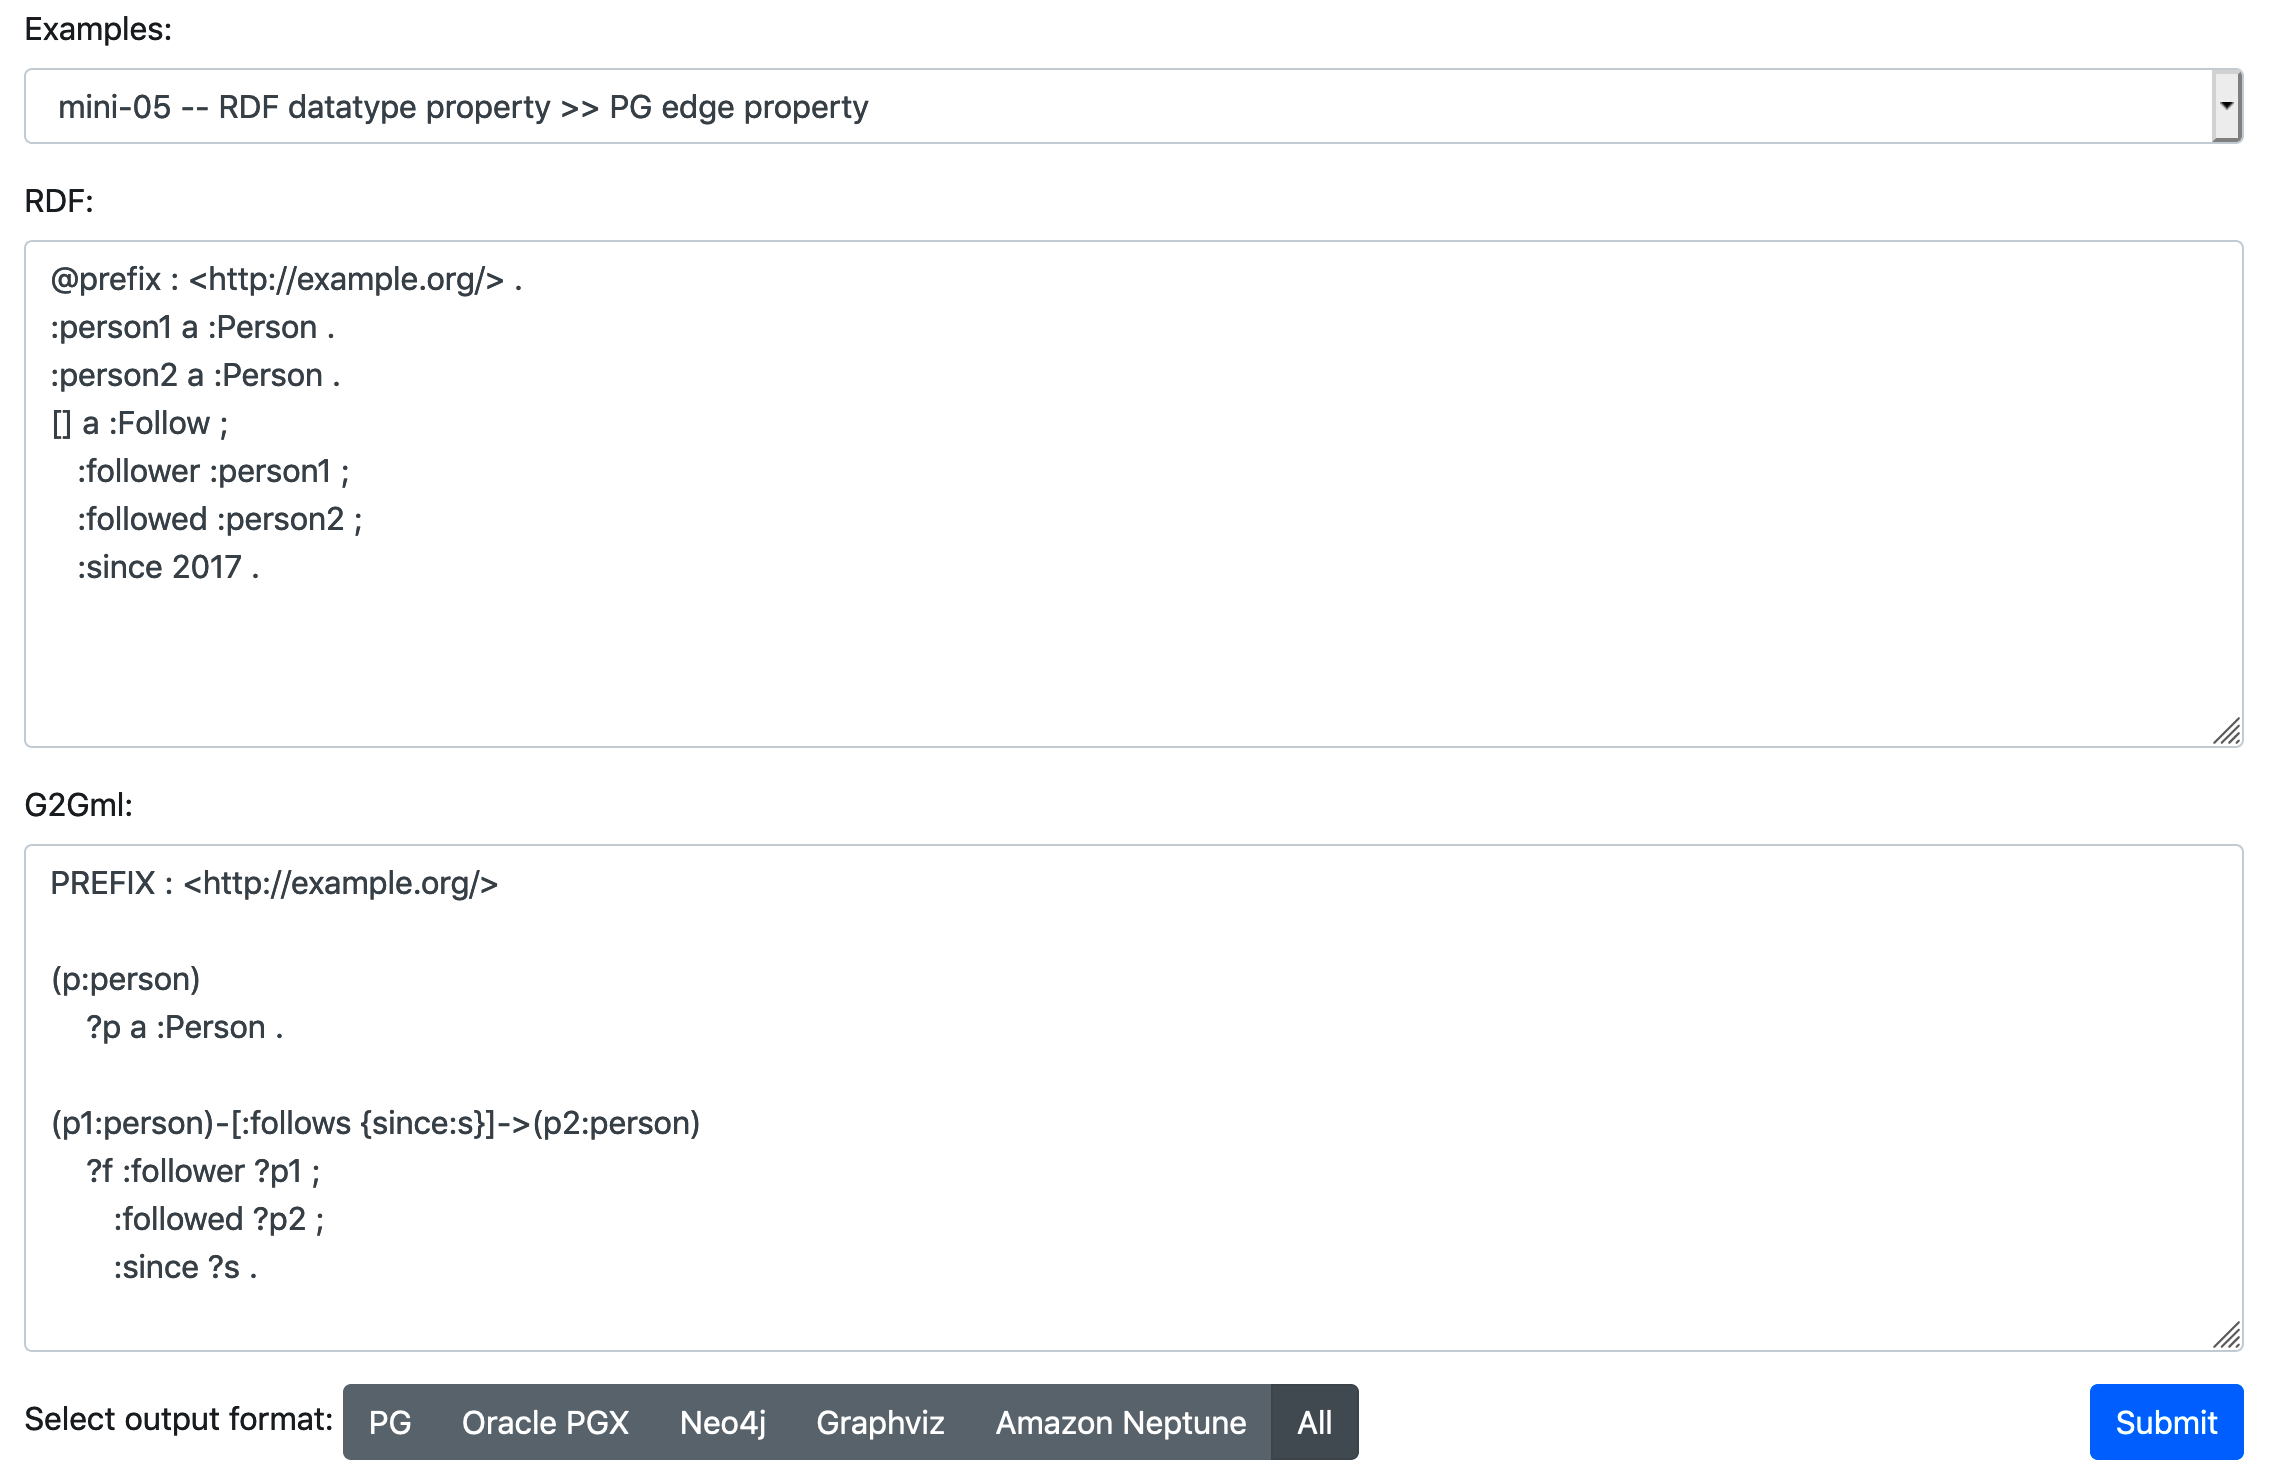
\includegraphics[width=1.0\textwidth]{sandbox.png}
\caption{G2G sandbox}
\label{fig:sandbox}
\end{figure}

\subsection{Graph Archive}
We created several G2GML mappings to extract public RDF from endpoint and construct knowledge graphs in PG format and resulting knowledge graphs as Graph Archive.

In the listed knowledge graphs, we compared the number of nodes and edges between RDF and property graphs.

%%%%%%%%%%%%%%%%%%%%%%%%%%%%%%%%

\section{Related Work}
Recently, the graph data have been attracting increasing attention, leading to plethora of database implementations. 
%So far, there have been implementations of graph databases on the basis of various data models and query languages. 
%So far, there are differences in data models and query languages based on the implementations of graph databases.
So far, there have been different data models and query languages for these graph database implementations.
Thus, there have been community-based activities for standardizing graph query language for interoperable use of property graph databases~\cite{angles3}. Similarly, standardization of the property graph model of various database implementations will enhance the interoperable use of graph data. In fact, there is a need for graph standardization in the community and graph data standardization was recently discussed in a W3C workshop~\cite{w3c}; there were similar proposals for property graph model and serialization~\cite{tomaszuk} including ours and it is noteworthy that the two independent approaches have converged to the similar solution. 
In particular, our serialization has implementation for some of the major database engines and also has a potential to cover further various implementations. %However, it requires developing a converter for each format. 
%This work provides a basis of an interoperable platform for creating, exchanging, and utilizing property graph data.
%Specifically, our model and serialization are independent of specific implementations and provides a basis 
%Specifically, it provides the basis for mapping of our G2GML mapping. 
The serialization formats independent of certain database implementations will increase the interoperability of graph databases and will make it easier for users to import accumulated graph data.
%In G2G mapping, PG format works as a gateway from RDF to property graphs.

As a preceding work for converting existing data into graph data, there was an effort to convert relational to graph databases~\cite{virgilio1}. 
However, given that RDF has now prevailed as a standardized data model in scientific communities, considering the mapping on the basis of the RDF model is crucial. There have been discussions about the interoperability of RDF and property graphs~\cite{hartig,angles4,das,thakkar} and efforts were made to develop methods to convert RDF into property graphs~\cite{tomaszuk1,virgilio}. However, considering the flexibility of what kind of information can be expressed by each edge in property graphs, a novel method for controlling the mapping is necessary.
To the best of our knowledge, this is the first attempt to develop a framework for controlled mapping between RDF and property graphs. 
Notably, the G2GML we have designed is a declarative mapping language. 
As a merit of the declarative description, we can concentrate on the core logic of mappings. In the sense that the mapping process generates new graph data on the basis of existing graph data, it has close relation to the semantic inference. Similar concept can be found in SPARQL CONSTRUCT queries. While the SPARQL CONSTRUCT clause defines mapping on the same data model, G2GML defines mapping between different data models. 
%Currently, it is limited to the mapping from RDF to property graphs, it can be extended to the mapping from property graph to RDF. However, if mapping includes the SPARQL pattern that are not declarative, it is not applicable for generating RDF triples.
Thus, G2GML can be considered as a specific extension of the SPARQL CONSTRUCT clause for generation or inference of property graph data.
%Future works include further analysis of the converted graph data on the database engines adopting the property graph model.

A previous work compared performance of Blazegraph and Neo4j. They concluded that RDF has advantage in terms of performance and interoperability.

\section{Conclusion}
Here we redefined the property graph model independent of specific graph database implementations and also proposed serialization formats based on the data model.
We further designed G2GML for mapping RDF graphs to property graphs and implemented a converter on the basis of G2GML.
Our data model and mapping framework will increase the interoperability of existing graph databases and make it easier for users to create, exchange, and utilize graph data.

\section*{Acknowledgements}
Part of the work was conducted through the BioHackathon meetings (\url{http://www.biohackathon.org}). We thank Yuka Tsujii for helping creating figures. We thank Ramona Roess for careful review of the manuscript and useful comments.

%
% ---- Bibliography ----
%
% BibTeX users should specify bibliography style 'splncs04'.
% References will then be sorted and formatted in the correct style.
%
\bibliographystyle{splncs04}
% \bibliography{mybibliography}
%
\begin{thebibliography}{8}

\bibitem{rdf}
RDF 1.1 Concepts and Abstract Syntax, W3C Recommendation 25 February 2014. \url{http://www.w3.org/TR/rdf11-concepts/}

\bibitem{dbpedia}
Lehmann, J., Isele, R., Jakob, M., Jentzsch, A., Kontokostas, D., Mendes, P. N., ... & Bizer, C. (2015). DBpedia–a large-scale, multilingual knowledge base extracted from Wikipedia. Semantic Web, 6(2), 167-195.

\bibitem{wikidata}
Vrandečić, D., & Krötzsch, M. (2014). Wikidata: a free collaborative knowledgebase. Communications of the ACM, 57(10), 78-85.

\bibitem{sparql}
SPARQL 1.1 Query Language, W3C Recommendation 21 March 2013. \url{http://www.w3.org/TR/sparql11-query/}

\bibitem{angles1}
Angles, R., Gutierrez, C.: An introduction to Graph Data Management. arXiv preprint arXiv:1801.00036 (2017)

\bibitem{angles2}
Angles, R., Arenas, M., Barceló, P., Hogan, A., Reutter, J., Vrgoc, D.: Foundations of Modern Query Languages for Graph Databases. ACM Computing Surveys (CSUR), 50(5), 68. (2017)

\bibitem{neo4j}
The Neo4j Graph Platform. \url{https://neo4j.com/}

\bibitem{pgx}
Oracle Labs Parallel Graph AnalytiX (PGX). \url{https://www.oracle.com/technetwork/oracle-labs/parallel-graph-analytix/overview/index.html}

\bibitem{neptune}
Amazon Neptune. \url{https://aws.amazon.com/neptune/}
 
\bibitem{hartig}
Hartig, O.: Reconciliation of RDF* and property graphs. arXiv preprint arXiv:1409.3288 (2014)

\bibitem{pgql}
van Rest, O., Hong, S., Kim, J., Meng, X., Chafi, H.: PGQL: a property graph query language. In Proceedings of the Fourth International Workshop on Graph Data Management Experiences and Systems, p. 7. ACM (2016)

\bibitem{angles3}
Angles, R., Arenas, M., Barceló, P., Boncz, P., Fletcher, G., Gutierrez, C., {\itshape et al.}: G-CORE: A core for future graph query languages. In Proceedings of the 2018 International Conference on Management of Data, pp. 1421--1432. (2018)

\bibitem{w3c}
W3C Workshop on Web Standardization for Graph Data. \url{https://www.w3.org/Data/events/data-ws-2019/}

\bibitem{tomaszuk}
Tomaszuk D., Angles R., Szeremeta L., Litman K., Cisterna D.:
Serialization for property graphs. International Conference: Beyond Databases, Architectures and Structures, pp. 57--69. (2019)

\bibitem{virgilio1}
De Virgilio, R., Maccioni, A., Torlone, R.: Converting relational to graph databases. In First International Workshop on Graph Data Management Experiences and Systems, p. 1. ACM (2013)

\bibitem{angles4}
Angles, R., Thakkar, H., Tomaszuk, D.: RDF and Property Graphs Interoperability: Status and Issues. Proceedings of the 13th Alberto Mendelzon International Workshop on Foundations of Data Management. (2019)

\bibitem{das}
Das, S., Srinivasan, J., Perry, M., Chong, E. I., Banerjee, J.: A Tale of Two Graphs: Property Graphs as RDF in Oracle. In EDBT, pp. 762--773. (2014)

\bibitem{thakkar}
Thakkar, H., Punjani, D., Keswani, Y., Lehmann, J., Auer, S.: A Stitch in Time Saves Nine--SPARQL querying of Property Graphs using Gremlin Traversals. arXiv preprint arXiv:1801.02911 (2018)

\bibitem{tomaszuk1}
Tomaszuk, D.: RDF data in property graph model. In Research Conference on Metadata and Semantics Research, pp. 104--115. (2016)

\bibitem{virgilio}
De Virgilio, R.: Smart RDF data storage in graph databases. In 2017 17th IEEE/ACM International Symposium on Cluster, Cloud and Grid Computing, pp. 872--881. IEEE (2017)

\bibitem{Alocci}
Alocci, D., Mariethoz, J., Horlacher, O., Bolleman, J. T., Campbell, M. P., & Lisacek, F. (2015). Property graph vs RDF triple store: A comparison on glycan substructure search. PloS one, 10(12), e0144578.


% \bibitem{ref_article1}
% Author, F.: Article title. Journal \textbf{2}(5), 99--110 (2016)

% \bibitem{ref_lncs1}
% Author, F., Author, S.: Title of a proceedings paper. In: Editor,
% F., Editor, S. (eds.) CONFERENCE 2016, LNCS, vol. 9999, pp. 1--13.
% Springer, Heidelberg (2016). \doi{10.10007/1234567890}

% \bibitem{ref_book1}
% Author, F., Author, S., Author, T.: Book title. 2nd edn. Publisher,
% Location (1999)

% \bibitem{ref_proc1}
% Author, A.-B.: Contribution title. In: 9th International Proceedings
% on Proceedings, pp. 1--2. Publisher, Location (2010)

% \bibitem{ref_url1}
% LNCS Homepage, \url{http://www.springer.com/lncs}. Last accessed 4
% Oct 2017
\end{thebibliography}
\end{document}
